\begin{abstract}
Adaptive strategy search creates an online multiple-testing problem: proposal
identities depend on earlier evaluations, monitoring horizons differ, and the
researcher may stop when evidence appears favorable.  SAFE-ALPHA separates an
arbitrary adaptive proposer from an executable ledger that fixes each strategy,
cost rule, bounded score, rank weight, and predictable e-process before its
first tested payoff.  Joint promotion and proposal-level evidence freezing
produce an irreversible set satisfying
\(\mathbb E[\sup_t\operatorname{FDP}(D_t)]\le q\) under arbitrary serial and
cross-strategy dependence.  Online e-BH is the testing engine; the contribution
is the financial deployment contract and its causal evaluation.  In 500
market-shaped sign-null replays at \(q=10\%\), false promotion occurs in 20
runs, while same-bar betting and repeatedly inspected nominal tests fail in
every run.  At planted annualized Sharpe \(1.5\) and correlation \(0.5\), the
original persistent rule attains power \(0.578\), versus \(0.479\) for a
matched terminal rule.  A development-frozen finite-campaign prior, daily
inspection, and prespecified three-bet mixture reach \(0.693\) on a new paired
holdout, versus \(0.572\) for the original schedule.  A locked U.S.\ industry
replay certifies the market control but none of 76 adaptive symbolic rules;
factor residualization removes the control certificate.  The evidence concerns
the committed bounded score, not raw-return alpha, drawdown, or profitability.
\end{abstract}

\keywords{adaptive strategy search, e-processes, false discovery rate, factor mining,
anytime-valid inference, backtest overfitting}

\begin{CCSXML}
<ccs2012>
 <concept>
  <concept_id>10010405.10010476</concept_id>
  <concept_desc>Applied computing~Economics</concept_desc>
  <concept_significance>500</concept_significance>
 </concept>
 <concept>
  <concept_id>10002950.10003624</concept_id>
  <concept_desc>Mathematics of computing~Probability and statistics</concept_desc>
  <concept_significance>500</concept_significance>
 </concept>
 <concept>
  <concept_id>10010147.10010178</concept_id>
  <concept_desc>Computing methodologies~Artificial intelligence</concept_desc>
  <concept_significance>300</concept_significance>
 </concept>
</ccs2012>
\end{CCSXML}
\ccsdesc[500]{Applied computing~Economics}
\ccsdesc[500]{Mathematics of computing~Probability and statistics}
\ccsdesc[300]{Computing methodologies~Artificial intelligence}

\maketitle

\section{Introduction}
\label{sec:introduction}

Consider a research agent that proposes a momentum rule, reads its backtest,
changes the lookback, compares the revision with other candidates, and
continues until something appears convincing.  A held-out period ceases to be
held out when its outcome shapes the next proposal, and a conventional test
loses its nominal interpretation when it is checked until rejection.  No
malicious data mining is required; multiplicity and optional stopping arise
from the architecture of the research process itself.

Recent systems use language models to propose, implement, debate, retrieve,
and evolve financial signals
~\cite{tang2025alphaagent,duan2025factormad,shi2026hubble,han2026quantaalpha,
huang2026beyond}.  Several enforce out-of-sample isolation or high terminal
test-statistic hurdles.  Those safeguards do not by themselves control error
across an adaptively growing stream that is inspected and stopped from the
complete research record.

SAFE-ALPHA assigns proposal and promotion to different components.  The
proposer may use the complete recorded past and may itself be stochastic,
language-model based, or adversarially persistent.  The ledger fixes the
candidate's formula, universe, execution lag, missing-data policy, cost model,
payoff transformation, and evidence rule before another payoff is observed.
The candidate then begins with unit evidence, and every material revision
receives a new identity.  A non-generative gate alone may add the strategy to
the certified set.

The protocol indexes both proposal time and market time.
Candidate \(j\) arrives at the adaptive research time \(\tau_j\), whereas its
evidence evolves over later market dates.  A terminal e-BH analysis presumes a
fixed decision horizon; preserving every interim peak is also invalid because
the running maximum of an e-process need not be an e-value
~\cite{tavyrikov2025carefree}.  SAFE-ALPHA instead allocates a summable budget
when the proposal arrives, applies the joint rule only to arrived candidates,
and freezes one e-valid value at the first joint promotion time.  The resulting
set is irreversible, which permits immediate deployment, yet its expected
worst realized false-discovery proportion remains bounded throughout the
research run.

SAFE-ALPHA makes three contributions distinct from the underlying e-BH rule.
First, it defines an executable financial-research contract in which proposal
identities and times may depend on the complete past, while the formula,
execution lag, costs, score, rank weight, and evidence rule are fixed before
the first tested payoff.  Second, it proves that joint promotion followed by
proposal-level freezing yields an irreversible set with
\(\mathbb E[\sup_t\operatorname{FDP}(D_t)]\le q\) under arbitrary serial and
cross-strategy dependence, and it gives pathwise power results for persistence
and denser inspection.  Third, it evaluates the complete causal protocol with
valid matched comparators, controlled timing violations, paired power and
delay experiments, and a public replay that separates the prespecified
control from adaptively selected rules.  Online e-BH, stopped e-values, and
worst-time FDR control are established statistical ingredients
~\cite{fischer2024online,wang2025stopped}.  The contribution here is the
deployment contract that makes those ingredients executable in adaptive
financial search.

\section{Relation to prior work}
\label{sec:related}

Multiple testing has long been central to empirical finance.  The Reality
Check and SPA address the best model in a fixed candidate family
~\cite{white2000reality,hansen2005spa}; the Deflated Sharpe Ratio and PBO are
retrospective diagnostics for selection and backtest overfitting
~\cite{bailey2014deflated,bailey2017pbo}; and the factor-zoo literature
documents why ordinary significance thresholds are too permissive
~\cite{harvey2016crosssection}.  These methods remain useful, but they target
a fixed or retrospectively enumerated search rather than hypotheses whose
identities, arrival times, and monitoring horizons depend on the evolving
research record.

Our gate builds on e-values~\cite{vovk2021evalues}.  e-BH controls FDR for
arbitrarily dependent e-values and includes a sequential-trader example
~\cite{wang2022false}; e-value procedures extend to online hypothesis arrival
~\cite{xu2024online,fischer2024online}; and stopped e-BH identifies the global
filtration required when evolving evidence streams are monitored jointly
~\cite{wang2025stopped}.  The 2026 online e-closure and donation framework
strictly improves baseline online e-BH on streams of fixed e-values
~\cite{xu2026closure}.  It does not directly supply the jointly stopped ledger
used here, in which every proposal carries an evolving global e-process, an
individual admission floor, and its own frozen promotion value.  We therefore
use the baseline whose stopped values can be audited proposal by proposal.
Our claim concerns neither e-BH nor worst-time FDR in isolation; it concerns
their deployment-safe composition with financial payoffs and the empirical
evaluation of the causal failures created by adaptive strategy search.

The need for a proposal-time budget can be seen without any finance-specific
distributional assumptions.  The following counterexample also explains why
running terminal e-BH after the agent decides to stop is not a valid repair.

\begin{proposition}[A random terminal family can have FDR one]
\label{prop:random-family}
Let every hypothesis be null and, independently for \(j\ge1\), set
\[
E_j=\begin{cases}j/q,&\text{with probability }q/j,\\0,&\text{otherwise}.
\end{cases}
\]
Every \(E_j\) is an e-value.  If proposal generation stops at
\(J=\inf\{j:E_j=j/q\}\), then \(J<\infty\) almost surely and ordinary
unweighted e-BH applied to \(E_1,\ldots,E_J\) rejects with FDR one.
\end{proposition}

\begin{proof}
Each expectation equals one, but independence and
\(\sum_jq/j=\infty\) imply that a success eventually occurs almost surely.
At that success, the one-rejection e-BH boundary for a family of size \(J\) is
\(J/q=E_J\).  Since all hypotheses are null, the resulting nonempty discovery
set has false-discovery proportion one.
\end{proof}

This construction does not invalidate terminal e-BH for a genuinely fixed
family and horizon.  It shows that the family size cannot be chosen by the
same evidence later submitted to the test, which is precisely what an
open-ended proposer would otherwise be allowed to do.

\section{The SAFE-ALPHA protocol}
\label{sec:method}

\subsection{One filtration and an immutable ledger}

Let
\((\Omega,\mathcal F,(\mathcal F_t)_{t\ge0},P)\) be a discrete-time filtered
probability space.  The global filtration contains all market observations,
agent inputs and outputs, candidate specifications, evidence streams, and
gate decisions available by \(t\).  Candidate \(j\) is proposed at a global
stopping time \(\tau_j\).  Its complete executable specification \(A_j\) is
\(\mathcal F_{\tau_j}\)-measurable, and only finitely many candidates have
arrived by any finite \(t\).  Later proposals may depend on all earlier
outcomes.  A revision of \(A_j\) is a new candidate, not a continuation of
\(j\).

For \(t>\tau_j\), let \(X_{j,t}\in[-1,1]\) be the one-period net performance
score generated by the committed execution and cost rules.  The null is
\begin{equation}
H_j:\quad
\mathbb E_P[X_{j,t}\mid\mathcal F_{t-1}]\le0
\quad\text{for every }t>\tau_j .
\label{eq:null}
\end{equation}
This is a conditional no-positive-drift null for the \emph{bounded score}.
It is stronger than nonpositive unconditional mean, nonpositive Sharpe, or a
zero factor-model intercept.  If returns are clipped to construct \(X\), the
certificate concerns the clipped score; it must not be described as a
certificate for the raw mean return.

Let \(\lambda_{j,t}\in[0,1]\) be \(\mathcal F_{t-1}\)-measurable and define
\begin{equation}
E_{j,t} =
\begin{cases}
1, & t\le\tau_j,\\
\displaystyle\prod_{s=\tau_j+1}^{t}
       (1+\lambda_{j,s}X_{j,s}), & t>\tau_j.
\end{cases}
\label{eq:eprocess}
\end{equation}
Under \(H_j\), \(E_j\) is a nonnegative supermartingale in the \emph{global}
filtration.  The distinction is essential.  A process valid only in its own
local history can cease to be valid when another strategy stream reveals
information used to stop it~\cite{wang2025stopped}.  Operationally, a signal
using date-\(t\) closes trades no earlier than the next implementable price;
data vintages, proposal timestamps, code hashes, random seeds, and cost inputs
are committed to the ledger before the corresponding outcome is observed;
Table~\ref{tab:contract} records these fields.

\begin{table}[t]
\caption{\textbf{The certification contract.} Every row is enforced by the
ledger rather than by the proposer.}
\label{tab:contract}
\centering
\small
\setlength{\tabcolsep}{3.4pt}
\begin{tabular}{p{.19\columnwidth}p{.72\columnwidth}}
\toprule
Stage & Committed or permitted information\\
\midrule
Proposal & Formula, universe, lag, costs, score, code hash; global past only\\
Execution & Point-in-time inputs through \(t-1\); realized payoff at \(t\)\\
Evidence & Post-proposal scores; predictable bet and scale only\\
Promotion & Joint weighted gate; evidence frozen on admission\\
Revision & New identifier, proposal time, weight, and unit evidence\\
\bottomrule
\end{tabular}
\end{table}

The predictability requirement has observable force.  Under a symmetric null
\(X_t\in\{-1,1\}\), choosing
\(\lambda_t=\tfrac12\mathbf1\{X_t=1\}\) after seeing \(X_t\) gives expected
one-step multiplier \(1.25\), not at most one.  This is the same-bar leakage
implemented in our ablation.  Likewise, retaining
\(\sup_{s\le t}E_{j,s}\) generally spends evidence more than once.  By
contrast, the first joint-promotion time below is a global stopping time, so
its single frozen value remains e-valid by optional sampling.

\subsection{Summable budget and irreversible gate}

Proposal \(j\) receives a nonnegative weight
\(\gamma_j\in\mathcal F_{\tau_j}\) with
\(\sum_{j\ge1}\gamma_j\le1\) almost surely.  Our default,
\begin{equation}
\gamma_j=\{j(j+1)\}^{-1},
\label{eq:gamma}
\end{equation}
supports an unbounded stream.  A data-dependent terminal family size cannot
safely replace this proposal-time budget.  We use the convention
\((q\gamma_jk)^{-1}=\infty\) when \(\gamma_j=0\), and impose the ledger-fixed
new-admission floor \(h=1/q\).  The floor is not needed for FDR control, but it
ensures that every promoted strategy has standalone evidence of at least
\(1/q\); without it, a weak-evidence candidate can become a passenger after a
large set of strong discoveries has lowered the joint threshold.

Let \(D_{t-1}\) be the finite set promoted before inspection \(t\).  The
finite adapted eligibility set obeys
\begin{equation}
D_{t-1}\subseteq\mathcal A_t\subseteq\{j:\tau_j<t\},
\label{eq:eligibility}
\end{equation}
which formally prevents an unproposed candidate, still carrying unit
evidence, from entering the gate.  Evidence for a promoted candidate is
frozen at its promotion time
\[
S_j=\inf\{t\ge\tau_j:j\in D_t\},\qquad
\widetilde E_j=E_{j,S_j}.
\]
For \(j\in\mathcal A_t\), form
\[
Z_{j,t}=
\begin{cases}
\widetilde E_j,&j\in D_{t-1},\\
E_{j,t},&j\in\mathcal A_t\setminus D_{t-1}.
\end{cases}
\]
For a proposed set size \(k\), define
\[
\mathcal C_t(k)=\left\{j\in\mathcal A_t:
Z_{j,t}\ge\max\!\left(h,\frac{1}{q\gamma_jk}\right)\right\}.
\]
The maximal feasible size and the new discovery set are
\begin{align}
k_t^\star
&=\max\!\left(\{0\}\cup
\left\{1\le k\le|\mathcal A_t|:|\mathcal C_t(k)|\ge k\right\}\right),
\label{eq:stepup}\\
D_t&=\mathcal C_t(k_t^\star),
\label{eq:discoveries}
\end{align}
where \(\mathcal C_t(0)=\varnothing\) and newly admitted evidence is then
frozen.  If \(d=|D_{t-1}|\), the induction invariant makes \(k=d\) feasible.
Hence
\(k_t^\star\ge d\), the joint threshold can only fall, and no promotion is
withdrawn.  If \(|\mathcal C_t(k_t^\star)|>k_t^\star\), the same set makes the
next integer feasible, contradicting maximality; thus
\(|D_t|=k_t^\star\).  Every old member satisfied its threshold when admitted,
and every new member satisfies the current one, which yields the invariant
\begin{equation}
j\in D_t\quad\Longrightarrow\quad
\widetilde E_j\ge\frac{1}{q\gamma_j|D_t|}.
\label{eq:selfconsistent}
\end{equation}
as well as \(\widetilde E_j\ge h\) for every member.  Freezing at \(S_j\) is
not the same as retaining \(\sup_{s\le t}E_{j,s}\): only evidence that passes
the joint gate at a declared inspection is remembered.

\section{Simultaneous error control}
\label{sec:theory}

Because the proposal itself is random, write \(N_j\) for the indicator that
the selected candidate is a true null under \(P\).  We require \(N_j\) to be
\(\mathcal F_{\tau_j}\)-measurable and, equivalently to
Eq.~\eqref{eq:null} on the null event,
\[
N_j\mathbf1\{\tau_j<t\}
\mathbb E_P[X_{j,t}\mid\mathcal F_{t-1}]\le0.
\]
This selective formulation permits the agent to choose \(A_j\) from the
global past.  It prohibits selecting \(A_j\) with the return intended to test
it.

\begin{theorem}[Persistent SAFE-ALPHA certificate]
\label{thm:main}
Suppose \(\tau_j\) is a global stopping time; \(A_j,N_j,\gamma_j\) are
\(\mathcal F_{\tau_j}\)-measurable; finitely many candidates arrive by each
finite \(t\); Eq.~\eqref{eq:null} holds on \(\{N_j=1\}\);
\(\lambda_{j,t}\) is predictable; \(\sum_j\gamma_j\le1\) almost surely; and
the finite adapted gate obeys Eq.~\eqref{eq:eligibility}, is nested, and
maintains Eq.~\eqref{eq:selfconsistent}.
Without independence assumptions beyond the stated conditional score null,
\begin{equation}
\mathbb E_P\!\left[\sup_{t\ge0}
\frac{\sum_{j\in D_t}N_j}{|D_t|\vee1}\right]\le q.
\label{eq:supfdr}
\end{equation}
Consequently
\(\mathbb E_P[\operatorname{FDP}(D_T)]\le q\) for every almost surely finite
global stopping time \(T\), including a stopping rule that uses all market
data, agent outputs, evidence, and portfolio results.
\end{theorem}

\begin{proof}
Predictability and the null condition give, on \(\{N_j=1,\tau_j<t\}\),
\[
\mathbb E_P[E_{j,t}\mid\mathcal F_{t-1}]
=E_{j,t-1}\{1+\lambda_{j,t}
\mathbb E_P[X_{j,t}\mid\mathcal F_{t-1}]\}
\le E_{j,t-1}.
\]
Thus \(N_jE_{j,t}\), viewed after \(\tau_j\), is a nonnegative
supermartingale starting at \(N_j\): conditioning on
\(\{\tau_j=r\}\) verifies the claim in the shifted filtration
\((\mathcal F_{\tau_j+n})_{n\ge0}\).  The promotion time \(S_j\) is global
because \(D_t\) is adapted.  For
\(\overline E_j=E_{j,S_j}\mathbf1\{S_j<\infty\}\), optional sampling at
\(S_j\wedge(\tau_j+m)\), followed by conditional Fatou as \(m\to\infty\),
yields
\begin{equation}
\mathbb E_P[N_j\overline E_j\mid\mathcal F_{\tau_j}]\le N_j.
\label{eq:selective-e}
\end{equation}
Indeed,
\(N_jE_{j,S_j}\mathbf1\{S_j\le\tau_j+m\}\) is bounded above by the stopped
variable and converges to \(N_j\overline E_j\), which supplies the
unbounded-stopping step.

For \(D_t\ne\varnothing\), Eq.~\eqref{eq:selfconsistent} implies pathwise
\[
\operatorname{FDP}(D_t)
\le q\sum_{j\in D_t}\gamma_jN_j\widetilde E_j
\le q\sum_{j\ge1}\gamma_jN_j\overline E_j.
\]
The right-hand side is independent of \(t\).  Taking the supremum, applying
Tonelli, conditioning on \(\mathcal F_{\tau_j}\), and using
Eq.~\eqref{eq:selective-e} give
\begin{align*}
\mathbb E_P[\sup_t\operatorname{FDP}(D_t)]
&\le q\sum_j\mathbb E_P[\gamma_jN_j\overline E_j]\\
&\le q\sum_j\mathbb E_P[\gamma_jN_j]\\
&\le q\mathbb E_P\!\left[\sum_j\gamma_j\right]\le q.
\end{align*}
The stopping-time statement follows because the FDP at \(T\) is bounded by
the displayed pathwise supremum.
\end{proof}

The persistence mechanism has two pathwise power properties.

\begin{proposition}[Containment under persistence and grid refinement]
\label{prop:terminal-containment}
At an inspection date \(t\), let \(R_t\) be the one-shot floor-augmented
weighted e-BH set computed from the unfrozen endpoints on the same eligible
set, with the same \(q\), weights, and floor.  Then \(R_t\subseteq D_t\).
Moreover, if one SAFE-ALPHA run inspects on a refinement of another run's
grid while all evidence paths and ledger fields remain fixed, its discovery
set contains the coarser run's set at every common inspection.
\end{proposition}

\begin{proof}
For terminal containment, take the union of the persistent run's old set and
\(R_t\).  Old members pass at the old set size and terminal members pass at
\(|R_t|\); every member therefore passes at the no-smaller union size because
the weighted boundary decreases with set size.  The union is feasible for
the maximal step-up rule.  For grid refinement, induct on the common
inspections and apply the same union argument to the refined run's old set
and the coarser run's newly feasible set.
\end{proof}

The same argument has a portfolio interpretation.  If all promoted
strategies receive equal gross sleeve weights, the fraction of gross capital
assigned to true nulls equals \(\operatorname{FDP}(D_t)\), so its expected
worst-time value is at most \(q\).  More generally, allocation shares
\(a_{j,t}\ge0\) satisfy the same bound if \(a_{j,t}=0\) outside \(D_t\),
\(\sum_ja_{j,t}\le1\), and
\(a_{j,t}\le q\gamma_j\widetilde E_j\).  A portfolio optimizer that discards
or reweights certificates without preserving this inequality receives no
capital-level FDR guarantee from the theorem.

The floor supplies a separate candidate-level reading.  On the null branch,
promotion implies \(E_{j,S_j}\ge1/q\), so conditional Markov and stopped
e-validity give
\(P(S_j<\infty\mid\mathcal F_{\tau_j})\le q\) on \(\{N_j=1\}\).  This
marginal statement does
not control the probability of any false promotion across the stream; that is
why the weighted joint gate remains necessary.

The default telescope is robust to an unbounded stream but need not match a
finite research campaign.  If a cap \(M\) is declared before the first
proposal, a valid finite-campaign prior is
\begin{equation}
\gamma_j^{(\eta)}=
\frac{1-\eta}{j(j+1)}+\frac{\eta}{M}\mathbf1\{j\le M\},
\qquad 0\le\eta<1.
\label{eq:campaign}
\end{equation}
Its infinite sum is one, so Theorem~\ref{thm:main} applies without change.
For \(\eta>0\), its one-discovery boundary improves on the telescope precisely
when \(j(j+1)>M\) and \(j\le M\); it sacrifices the earliest ranks and makes
post-cap boundaries larger by \(1/(1-\eta)\).  The cap is a ledger field, not
the realized proposal count, and unused uniform mass is never reclaimed.

The main proof also quantifies implementation error.  If stopped null
evidence instead satisfies
\(\mathbb E[N_j\overline E_j\mid\mathcal F_{\tau_j}]
\le N_jc_j\), where \(c_j\ge1\) is fixed at proposal time and
\(\sum_j\gamma_jc_j\le C\), the same calculation yields
\begin{equation}
\mathbb E[\sup_t\operatorname{FDP}(D_t)]\le qC.
\label{eq:validity-debt}
\end{equation}
Thus a bounded evidence inflation has an explicit validity debt, while
dividing each stream by a predictable upper bound on its cumulative inflation
restores the level-\(q\) statement.

\section{Empirical design}
\label{sec:experiments}

\subsection{Public-data strategy stream}

We use daily value-weighted returns for the 30 U.S.\ industry portfolios and
the daily risk-free rate from the Kenneth French Data
Library~\cite{french2026data}.  The report window is January 3, 2007 through
May 29, 2026; five prior years initialize proposal scores.  Download hashes
and the complete processed panel are recorded.  Because the current library
reconstructs historical series after CRSP updates, this block is an auditable
economic illustration, not a point-in-time claim that historical alpha was
discovered.

The fixed symbolic grammar contains 89 executable candidates: one
equal-weight industry-market sleeve; 48 weekly or monthly cross-industry
momentum and reversal spreads; 24 monthly low- or high-volatility spreads;
and 16 weekly or monthly time-series momentum or reversal overlays.  Signals
use 21, 63, 126, or 252 trading-day lookbacks and are lagged before execution.
Long-short rules have unit gross exposure.  Turnover is half the
\(\ell_1\) change in pretrade-to-target risky weights, charged at 2, 5, or 10
basis points per unit.  Risky weights drift after each return; residual capital
earns the risk-free rate.  Displayed sleeve allocations are restored daily
from their drifted weights, and both within-sleeve and allocation turnover are
charged under the declared half-\(\ell_1\) convention.

To isolate the statistical layer from model-specific prompting, the main
experiment uses a transparent adaptive proposer.  The market sleeve is a
predeclared positive control assigned the first budget slot.  At experiment
start and on the first trading day of each subsequent quarter, the proposer
selects the unproposed rule maximizing its trailing five-year annualized
Sharpe minus \(0.20\) times its largest absolute correlation with earlier
proposals.  This yields 76 adaptive symbolic proposals plus the control (77
total).  The replay therefore evaluates the certification layer, not the
proposal quality of a particular LLM.  A generative proposer can use the same
interface only if every executable output is committed before its first scored
payoff.

For certification, net return \(R_{j,t}^{\rm net}\) becomes
\[
X_{j,t}=\operatorname{clip}\!\left(
\frac{R_{j,t}^{\rm net}}
{4\max\{\widehat\sigma_{j,t-1},10^{-6}\}},-1,1\right),
\]
where \(\widehat\sigma_{j,t-1}\) is a lagged 63-day volatility estimate with a
lagged expanding fallback.  The fixed proposal-time bet is the mean of up to
1,260 available prior bounded scores divided by their second moment, clipped
to \([0.01,0.50]\); first-date histories contain 1,239 scores after scale
initialization.  On the frozen panel, scale multiples 2, 4, and 8 clip
respectively \(6.05\%\), \(0.318\%\), and \(0.0099\%\) of finite scores; the
corresponding fractions of proposal-time bets at the upper cap are zero,
zero, and \(13.0\%\).  The primary multiple of 4 therefore keeps clipping
below \(0.4\%\) without activating the upper betting cap, while the sensitivity
analysis reports the two alternatives.  We use Eq.~\eqref{eq:gamma},
\(q=0.10\), and inspect every
fifth trading day.  At 5 and 10 basis points we rebuild candidate return,
drifted-weight, and turnover paths; the proposal ledger, 2-basis-point scale
reference, and bets remain fixed.

\subsection{Identification of validity and power}

Historical returns do not reveal which nulls are true.  We therefore separate
calibration from economics.

\textbf{Cross-sectional sign null.}
For each of 500 replications, an independent Rademacher sign
\(\varepsilon_t\) multiplies the entire 89-dimensional realized score vector
\(x_t\) on each date.  This leaves \(x_tx_t^\mathsf T\), and hence all
same-date cross-strategy dependence and heteroskedastic magnitudes, unchanged.
Because \(\varepsilon_t\) is independent of the signed past,
\(\mathbb E[\varepsilon_tx_{j,t}\mid\mathcal F_{t-1}]=0\), even when the
candidate index was selected adaptively from that past.  The experiment does
not preserve serial sign predictability and is not presented as a complete
market simulator.  The proposer reselects adaptively
every 63 trading days after assigning the signed market control to the first
slot, until the ledger contains 77 proposals.  We compare SAFE-ALPHA with
(i) an illegal same-bar bettor that wagers only after seeing that the current
score is nonnegative, (ii) one-sided 5\% \(t\)-tests inspected every week
after 63 observations, and (iii) one unadjusted one-sided 5\% test after a
252-day holdout for each horizon-eligible proposal (74 of 77).  The last
comparator diagnoses ignored cross-proposal multiplicity; it is not a
multiplicity-adjusted fixed split.

The wild-sign construction preserves realized same-date dependence and
volatility magnitudes but removes serial sign structure.  We therefore add a
fixed synthetic null with standardized Student \(t_3\) innovations, a
predictable common GARCH-style scale recursion, cross-candidate correlation
\(0.5\), and clipping to the same score range.  In both null designs every
procedure sees the identical candidate paths.  A nine-point grid from
\(q=0.01\) through \(0.20\) describes sensitivity around \(q=0.10\) on the
same paths.

\textbf{Paired planted alternatives.}
Each replication has 80 bounded Gaussian-score candidates, of which 16 have
positive drift, 504 burn-in days, and a common 1,260-day proposal/evaluation
period.  The first proposal has the largest burn-in sample mean; every later
proposal is the remaining candidate with the largest trailing annualized
Sharpe, with no diversity penalty.  Up to 50 candidates are selected at
15-day intervals, so strict post-proposal monitoring ranges from 1,259 days
for the earliest proposal to 524 for the latest.  The reported planted Sharpe
is the nominal pre-clipping mean-to-volatility ratio.  It ranges from
\(0.50\) to \(3.00\) in increments of \(0.25\), at equicorrelations zero and
\(0.5\), with 250 replications in every cell.  SAFE-ALPHA and the matched
terminal weighted e-BH comparator receive the same scores, proposal order,
proposal-time bets, spending weights, and raw e-process paths; only the
decision schedule differs.  The terminal rule reads the untouched endpoints
once, whereas SAFE-ALPHA inspects every five days and freezes only promoted
copies.  Ordinary terminal BH, uncorrected 5\% tests, and the five largest
post-proposal sample means remain diagnostic comparators.  We report realized
FDP, end-to-end power over all 16 planted alternatives, proposal recall,
conditional gate power, and delay from proposal to decision.

\textbf{Prospective power extension.}
No market outcome entered power-design selection.  On two recorded 300-path
development banks, we chose Eq.~\eqref{eq:campaign} with \(M=50\),
\(\eta=.75\), daily inspection, and the equal arithmetic mixture of three
e-processes whose proposal-time bets are
\(\min\{.5,m\widehat\lambda_j\}\) for \(m\in\{1,2,4\}\).  Such fixed mixtures
are established betting constructions, not a novelty claim
~\cite{waudbysmith2024betting,kaufmann2021mixture}.  We froze this design and
then generated six new 250-path cells at Sharpes 1, 1.5, and 2 and correlations
zero and .5.  The original public replay remains on the telescope, the fixed
plug-in bet, and five-day inspection.  A valid conservative comparator promotes
proposal \(j\) only when \(E_{j,t}\ge(q\gamma_j)^{-1}\); conditional Ville and
\(\sum_j\gamma_j\le1\) give FWER at most \(q\).  Every comparator receives the
same score paths, proposal order, weights, betting components, and inspection
grid permitted by the comparison.

\textbf{Economic and selection diagnostics.}
We report an ungated top-five policy reselected quarterly from the trailing
five years; a fixed split trained from 2002 through 2010, validated from 2011
through 2014, and tested from 2015 through 2026; and a deliberately optimistic
full-sample top five.  For the certified sleeve we estimate post-certification
CAPM and Fama-French five-factor plus momentum intercepts by OLS with
heteroskedasticity and autocorrelation consistent standard errors using five
lags.  A second gate predictably removes those six factor returns with rolling
betas estimated only from the previous 1,260 dates and at least 252
observations.  Across the 74 symbolic proposals with a complete one-year
future window, we compare the five-year selection Sharpe with the next-year
Sharpe and bootstrap the median change.  Finally, we compute White's Reality
Check, Hansen's SPA with consistent recentering, 1,999 stationary-bootstrap
draws, and mean block length 20, the Deflated Sharpe Ratio, and ten-block
CSCV/PBO.  The Reality Check retains its circular-block convention, so its
p-values are not numerically interchangeable with SPA.  These fixed-search
diagnostics test economic interpretations that the sequential score
certificate itself does not imply.

\section{Results}
\label{sec:results}

\begin{figure*}[t]
\centering
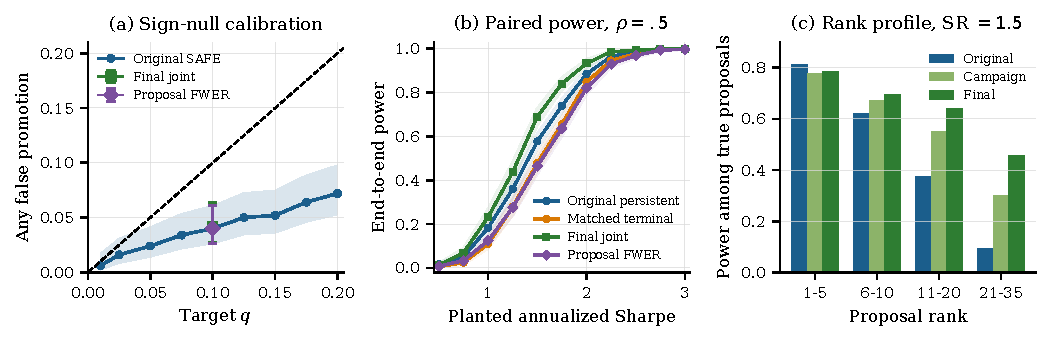
\includegraphics[width=.98\textwidth]{figures/calibration_power.pdf}
\Description{Panel a plots sign-null false-promotion probability against the
target level. Panel b plots end-to-end power for the original persistent,
matched terminal, final joint, and proposal-wise FWER procedures. Panel c
compares power by proposal-rank bin.}
\caption{Calibration and paired power.  Panel (a) uses 500 sign-null paths;
the curve is the original protocol and the two \(q=.10\) points use the final
design.  Panel (b) uses 250 paired paths per effect at \(\rho=.5\); shaded
regions are seed-level 95\% intervals.  Panel (c) uses the newly seeded central
holdout and counts only true proposals within each rank bin.}
\label{fig:calibration-power}
\end{figure*}

\subsection{Calibration, persistence, and power}

The original procedure makes at least one false promotion in 20 of 500
same-date sign-null runs, probability \(0.040\) with 95\% Wilson interval
\([0.026,0.061]\).  Across nine levels, the curve rises from \(0.006\) at
\(q=.01\) to \(0.072\) at \(q=.20\) and remains below the diagonal.  Under
the final campaign and betting design, the corresponding \(q=.10\) probability
is \(0.042\), interval \([0.028,0.063]\), versus \(0.040\) for proposal-wise
FWER.  The heavy-tailed volatility null gives \(0.034\) for the original gate
and \(0.020\) for the final design.
By contrast, same-bar betting and repeatedly inspected 5\% tests promote in
every sign-null run; separate one-year tests across 74 proposals promote in
\(94.4\%\).  These gray-box ablations identify timing and multiplicity failures,
whereas the terminal e-BH and proposal-wise FWER procedures are valid
comparators.

At annualized Sharpe \(1.5\) and \(\rho=.5\), the original persistent rule has
power \(0.578\), versus \(0.479\) for matched terminal weighted e-BH.  The
paired gain is \(0.099\), with interval \([0.084,0.113]\), and persistence
never loses on any of the 250 matched paths, as
Proposition~\ref{prop:terminal-containment} predicts.  Mean decision delay
among detected alternatives is 684 trading days for persistence and 1,183
for terminal analysis; the detected subsets differ, so this delay contrast is
descriptive rather than a paired causal estimate.

The newly seeded holdout confirms the prospective power extension.  At the
same central effect, the final design reaches \(0.693\), compared with
\(0.645\) for campaign weights and daily inspection alone and \(0.572\) for
the original schedule.  Its paired gains are \(0.048\), interval
\([0.034,0.062]\), over the campaign-only design and \(0.121\), interval
\([0.104,0.137]\), over the original.  Against proposal-wise e-alpha-spending
on a dense paired grid, joint power is \(0.690\) versus \(0.465\), a gain of
\(0.226\) with interval \([0.208,0.243]\); the joint gate wins on 225 paths
and ties on 25.  The gain is rank-specific.  Relative to the original, final
power changes from \(0.812\) to \(0.785\) at ranks 1--5, but rises from
\(0.623\) to \(0.695\) at ranks 6--10, from \(0.375\) to \(0.641\) at ranks
11--20, and from \(0.091\) to \(0.457\) at ranks 21--35.  This is the intended
finite-campaign tradeoff, not uniform dominance.

\subsection{Locked public replay and selection decay}

The rank-one market sleeve is a prespecified pipeline control rather than an
adaptively discovered alpha.  It crossed its boundary on January 19, 2018 at
frozen evidence \(20.087\), showing that the proposal, evidence, promotion,
and next-bar deployment path can operate on financial data.  The substantive
discovery result is negative: none of 76 adaptively proposed symbolic rules
was certified at \(q=0.10\), and predictable six-factor residualization
produced no certificate at all.  We therefore read the replay as evidence
about selection control in adaptive strategy search, not as evidence that
SAFE-ALPHA discovers factor-adjusted alpha.  The market control still crossed
at 5 and 10 basis points, with the 10-basis-point crossing delayed by one
week.

The ledger entry makes the joint rule concrete.  At the January 19 inspection,
the market control had \(\gamma_1=1/2\), so a one-member discovery set required
\[
E_{1,t}\ge\max\{1/q,(q\gamma_1)^{-1}\}
=\max\{10,20\}=20.
\]
Its current value was \(20.087\), while no other eligible candidate supported
a larger feasible set.  The gate froze that value, recorded the code and cost
specification used to obtain it, and began portfolio deployment on the next
tradable date rather than earning the triggering return twice.
Figure~\ref{fig:evidence-path} records the corresponding weighted paths.

\begin{figure*}[t]
\centering
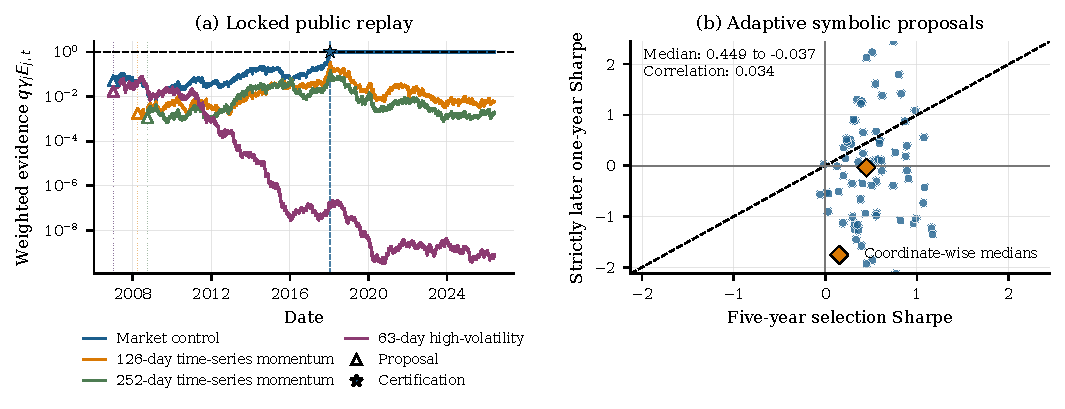
\includegraphics[width=.98\textwidth]{figures/evidence_path_repaired.pdf}
\Description{Panel a shows weighted evidence paths for the market control and
three symbolic proposals. Panel b plots five-year selection Sharpe against
strictly later one-year Sharpe for 74 symbolic proposals.}
\caption{Locked public replay and selection decay.  Panel (a) initializes each
path at unit evidence on its proposal date and updates it strictly later; the
market path is frozen at its crossing.  The three symbolic paths are selected
for display by their recorded maxima, which never enter the gate.  Panel (b)
uses the 74 symbolic proposals with a complete 252-day future window; the
diamond marks the coordinate-wise medians.}
\label{fig:evidence-path}
\end{figure*}

Deployment begins one trading day after promotion.  From January 22, 2018
through May 29, 2026, the market control earns \(9.96\%\) annualized net
excess return at \(19.77\%\) volatility, Sharpe \(0.504\), and maximum
drawdown \(-38.70\%\).  These are properties of a broad market sleeve, not
evidence of mined alpha; the large drawdown also shows why a score certificate
is not a risk guarantee.

\begin{table}[t]
\caption{Discovery and fixed-family diagnostics.  ``All'' includes the
prespecified market control.  Reality Check and SPA test different objects
from the sequential conditional-score null.}
\label{tab:diagnostics}
\centering
\small
\setlength{\tabcolsep}{2.8pt}
\begin{tabular}{lrr}
\toprule
Diagnostic & Adaptive & All\\
\midrule
Primary certificates & 0 of 76 & 1 of 77\\
Factor-residual certificates & 0 of 76 & 0 of 77\\
Median selected / future SR & .449 / -.037 & ---\\
Reality Check \(p\) & .190 & .022\\
SPA \(p\) & .146 & .157\\
\bottomrule
\end{tabular}
\end{table}

The factor evidence in Table~\ref{tab:diagnostics} clarifies the certificate's
interpretation.  Over 2,100 post-certification dates, the market sleeve has a
CAPM beta of \(0.941\); the six-factor regression explains \(95.9\%\) of its
variation and estimates a market beta of \(0.948\).  Both intercepts are
negative and statistically insignificant.  When candidate returns are
predictably residualized with betas fitted only through the preceding date,
the gate certifies no strategy.  The sole primary certificate is therefore a
broad market positive control under the committed bounded score, not evidence
of factor-adjusted alpha.

The proposal ledger displays the selection effect that a terminal winner
table would conceal.  Among 74 symbolic proposals with a complete 252-day
future window, median annualized Sharpe falls by \(0.512\), 70.3\% perform
worse after proposal, only 48.6\% remain positive, and the correlation between
selection and future Sharpe is \(0.034\).  An independent proposal-resampling
95\% percentile interval is \([0.398,0.754]\), but it is descriptive because
the proposals overlap.  White's Reality Check rejects on the full 89-rule
panel, but not
after removing the market control or restricting attention to adaptive
proposals; consistently recentered SPA does not reject in either the full or
adaptive family.  Although these procedures test different nulls, they point
in the same descriptive direction once the prespecified market sleeve is
distinguished from the mined symbolic rules.

One-at-a-time design changes reveal where the negative result is stable and
where the estimand changes.  At \(q=0.05\) no candidate is certified; at
\(q=0.20\) the market control and one monthly time-series momentum rule cross.
Daily inspection preserves the primary market certificate, inspection every
21 days misses its transient valid crossing, and moving the market control
from budget rank one to ranks 5, 10, or 20 produces no certification.  Scaling
returns by two lagged volatilities yields three promotions, while scaling by
eight yields none.  These are not interchangeable tuning choices after the
fact: they define different ledger-fixed scores, budgets, and inspection
opportunities, which is why the ledger records them explicitly.

\section{Audit and replication record}
\label{sec:reproducibility}

The released strategy catalog and proposal, evidence, and certification
ledgers identify every empirical decision, while tests enforce strict
post-proposal updating and next-bar deployment.  SHA-256 digests cover inputs,
code, and reported outputs.  Replication-level records retain the seed map for
the 5,500 paired evaluation paths together with null, sensitivity, and
portfolio accounting results.

\FloatBarrier
\section{Limitations and scope}
\label{sec:limitations}

The theorem applies to Eq.~\eqref{eq:null}, not to a weaker unconditional
alpha null.  Our bounded transformation changes the estimand, and a production
system seeking a raw-return claim should instead use an e-process justified
by explicit tail or conditional-moment assumptions.  FDR controls membership
of the certified set; it does not guarantee profitability, diversification,
market capacity, CVaR, or low drawdown.  A downstream optimizer must obey the
allocation constraint above if capital-weighted false exposure is the target.

The deterministic proposer is an identification choice: the study isolates
the gate rather than benchmarking language models, so it does not establish
how proposal quality changes under a particular LLM.  The public industry
series are nontradable research
portfolios and not archival point-in-time vintages; costs omit impact,
borrowing, and capacity.  Planted alternatives impose persistent constant
drift in a stationary Gaussian-score design, not alpha decay, regime change,
or crowding.  Finally, every summable rank prior trades power across proposal
positions.  The finite-campaign schedule improves middle and late ranks
within its declared cap but weakens the earliest ranks and the post-cap stream.
Weak persistent effects can still require long monitoring histories.

\section{Conclusion}
\label{sec:conclusion}

SAFE-ALPHA reserves promotion for a statistical gate that reads only
post-proposal payoffs and freezes evidence at a joint crossing.  Under the
stated conditional null, the persistent set controls worst-time expected FDP
despite dependence and adaptive stopping, while a declared campaign prior,
daily inspection, and a fixed betting mixture raise central holdout power by
12.1 percentage points relative to the original schedule.  The public replay
reaches a deliberately restrained conclusion: the prespecified market control
crosses, none of 76 adaptive symbolic rules does, and factor residualization
removes the control certificate.  The practical value is therefore not a
promise of profitable alpha, but a defensible separation between attractive
research output and evidence strong enough to justify deployment.
